
\section{Understanding the Potential Translation Ability of LLMs}
\label{sec:finetuning}
In this section, we first assess the overall translation performance of \method by comparing it to few-shot in-context learning\footnote{We randomly select 8 examples from the FLORES-101 dev split as the demonstration for ICL. Random selection strategy is shown to be good enough in many previous works~\citep{vilar-etal-2023-prompting,zhu2023multilingual}. The template we use for ICL is 
 <src\_text> = <tgt\_text>, which shows good performance according to~\citet{zhu2023multilingual}.}. We then present a detailed analysis of how the corpus for \method influences the translation quality.


\begin{figure*}[t]
  \centering
  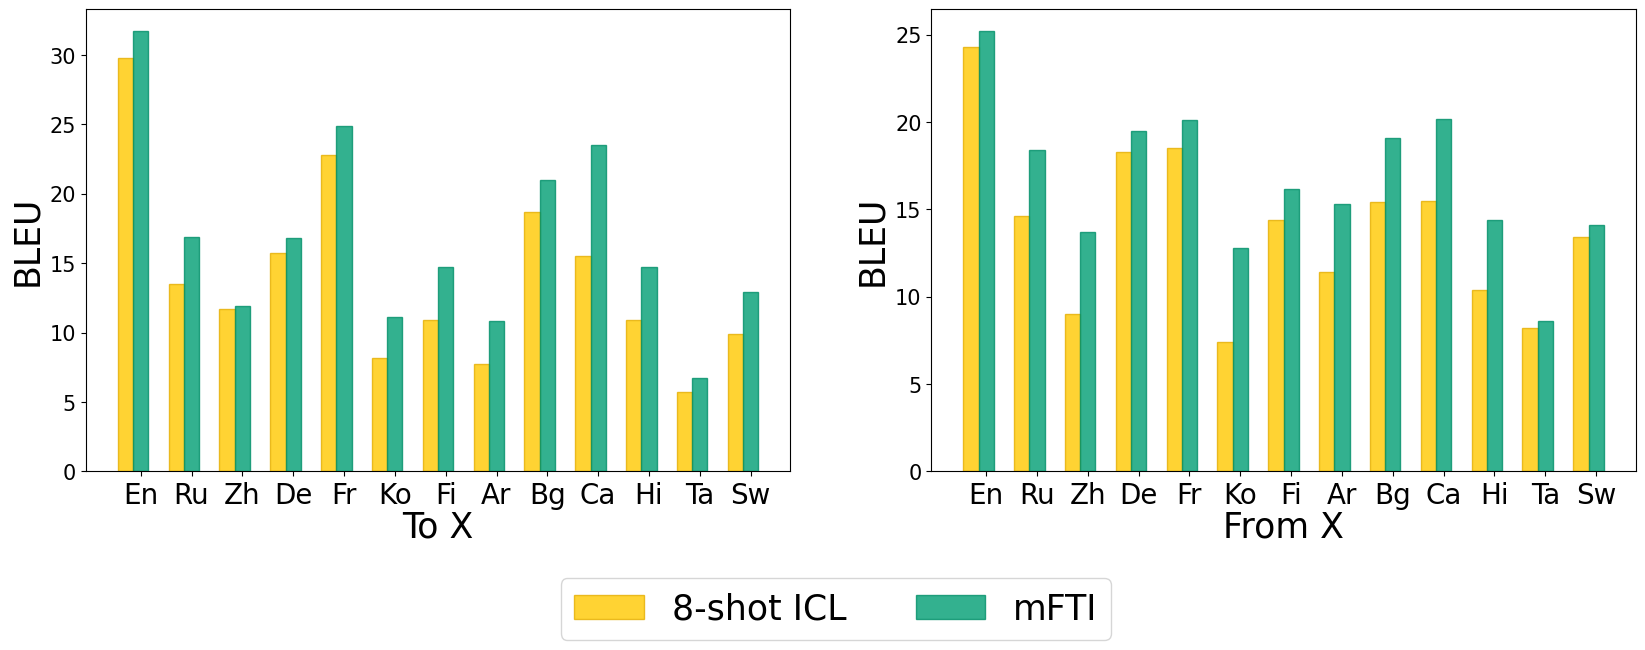
\includegraphics[width=1.0\linewidth]{figs/main_results.png}
  \caption{Translation performance of 8-shot ICL and \method using 1000 sentences per language pair. Languages are ordered by the data amount in the pretraining corpus.}
  \label{fig:main_results}
\end{figure*}

\subsection{Translation Ability of LLMs}



We finetune XGLM on 156 language pairs spanning all 13 languages. Since our goal is to elicit the translation ability of LLMs using a small number of examples, we limit the number of parallel sentences to 1000 per language. 


\paragraph{\method Better Elicits Translation Ability than Few-shot ICL.} Figure \ref{fig:main_results} shows the average BLEU for translation to and from language X, respectively. Full results on each langauge direction can be found in Appendix~\ref{appendix: full results}.
%BLEU scores for different language pairs are shown in Appendix ~\ref{appendix: full results}. 
It is clear that \method leads to better translation performances than 8-shot ICL for all language pairs (3 BLEU on average). For some languages, the gap is up to 8 BLEU (e.g. translating into Catalan). This demonstrates the effectiveness of \method in eliciting LLM's translation ability. It also shows that LLMs have a greater potential for multilingual translation than we saw with ICL~\citep{lin-etal-2022-shot}. 

Even for translating to and from English, \method still outperforms 8-shot ICL, but with a much smaller gap. This indicates that LLMs with ICL are better at performing tasks that involve English rather than other languages, but they still have the potential to perform even better. 

\begin{table}[t]
\centering
\begin{tabular}{@{}rcc@{}}
\toprule
\multicolumn{1}{l}{}                           & \textbf{To X} & \textbf{From X} \\ \midrule
\multicolumn{1}{l}{\textbf{Data Amount in Pretraining}} & 0.39          & 0.36            \\ \midrule
\multicolumn{3}{l}{\textbf{Similarity To English}}                                        \\
\textit{Geography}                                      & 0.93          & 0.87            \\
\textit{Syntax}                                         & 0.85          & 0.80            \\
\textit{Phylogeny}                                      & 0.71          & 0.75            \\
\textit{Phonology}                                      & 0.50          & 0.49            \\
\textit{Inventory}                                      & 0.51          & 0.41            \\ \bottomrule
\end{tabular}
\caption{Spearman correlation between average translation performance (in BLEU) and possible influence factors (data amount in pretraining, similarity to English). The performance of translating to and from language X is calculated separately.}
\label{tab:factor}
\end{table}

\paragraph{XGLM is still an English-centric Model.}
The translation performance for each language varies greatly. Considering that the number of sentences used in \method is the same for each language, one may suspect that the translation performance of each language largely depends on the amount of its pretraining data. For this reason, the languages in Figure \ref{fig:main_results} are listed in descending order of their data amount in the XGLM pretraining. However, there are clear fluctuations. For example, Russian and Chinese are the two languages with the largest portion of pretraining data other than English, but their translation performance is much worse than some other languages such as French. 

We calculate the Spearman correlation between the translation performance and possible influence factors, namely data amount in pretraining and similarity to English. For data amount, we use the size of the pretraining corpus reported in \citet{lin-etal-2022-shot}. For similarity to English, we adopt the lang2vec\footnote{\url{https://github.com/antonisa/lang2vec}}, which is a toolkit for querying the URIEL typological database, to get each language's feature vector of different perspectives including  \textit{geography}, \textit{syntax}, \textit{phylogeny}, \textit{phonology} and \textit{inventory}\footnote{We refer readers to~\citet{littell-etal-2017-uriel} for details on how the feature vector is obtained.}. %use the cosine similarity of averaged token representations produced by XGLM-7B. 



As shown in Table~\ref{tab:factor}, the translation performance indeed has a positive correlation with data amount in pretraining (0.39/0.36). However, the similarity between a specific language and English plays a more important role in determining the final translation performance. All considered features demonstrate a higher correlation coefficient than the data amount in pretraining. This indicates that XGLM is still a predominantly English-centric model. Based on these observations, we suggest taking the relation between different languages into consideration when collecting and sampling data for pretraining multilingual LLMs.

\begin{figure}[t]
\centering
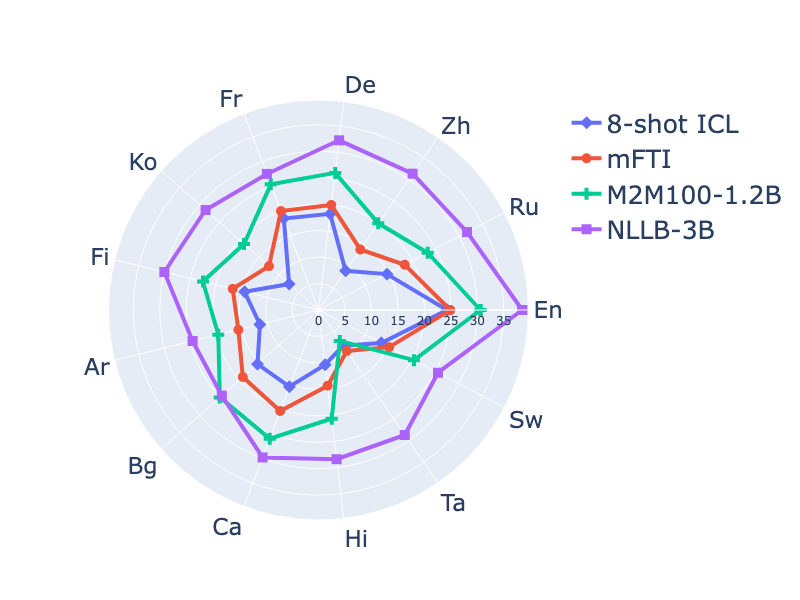
\includegraphics[width=0.95\linewidth]{figs/supervised.png}
\caption{Comparison of \method with conventional supervised machine translation models. Performances are evaluated in BLEU. }
\label{fig:supervised}
\end{figure}

\begin{figure}[t]
\centering
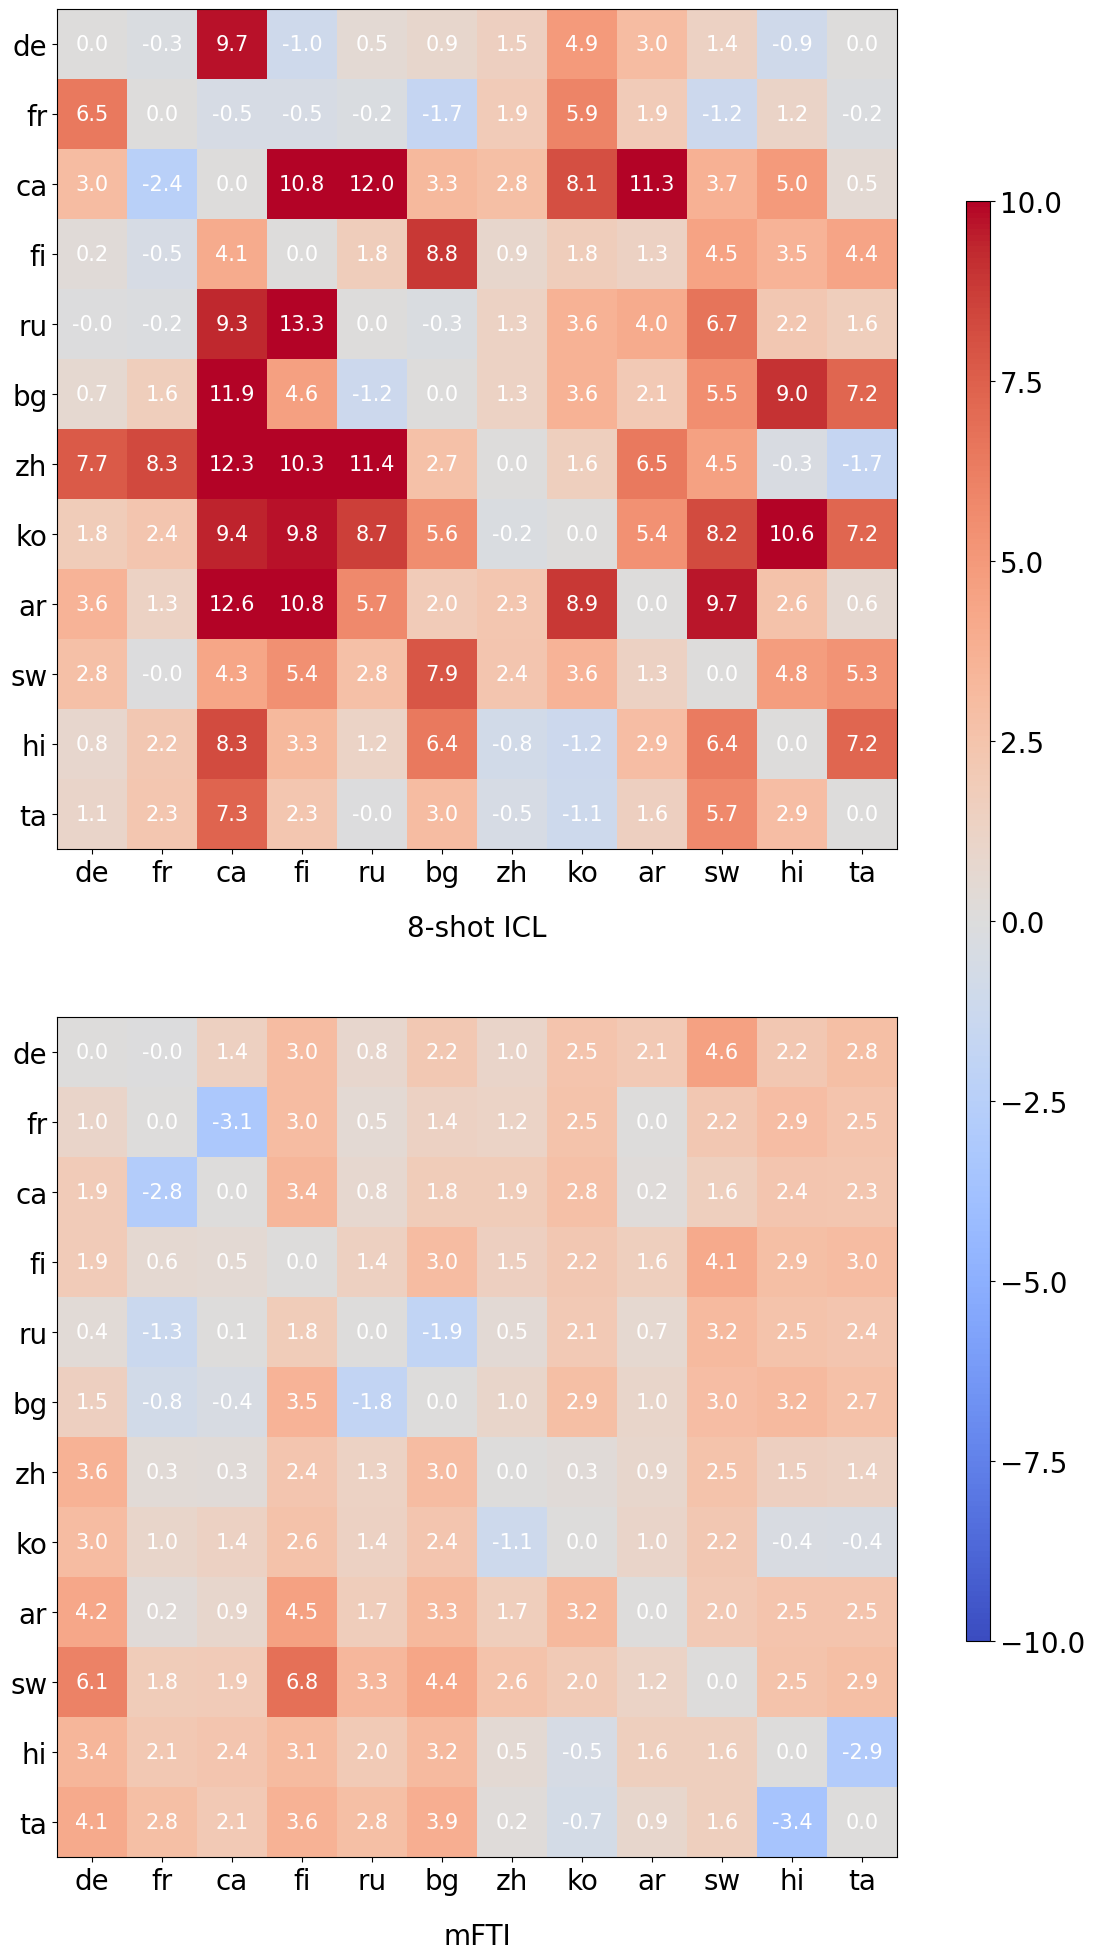
\includegraphics[width=0.95\linewidth]{figs/pivot.png}
\caption{Changes of BLEU score after pivoting through English for 8-shot ICL and \methodend.}
\label{fig:pivot}
\end{figure}



\paragraph{It is not trivial for LLM-based models to outperform conventional supervised MT models.} To better posit the performance of \method, we compare it with two conventional supervised MT models, i.e., M2M-1.2B~\citep{m2m100} and NLLB-3B~\citep{nllb} model, in Figure~\ref{fig:supervised}~\footnote{We also include the performance evaluated by COMET in Appendix~\ref{sec:supervised_comet}.}. We can see that despite that \method significantly improves over 8-shot ICL and sometimes achieves comparable performance to M2M-615M, it still lags behind the stronger NLLB-3B by a large margin, rendering the challenge to adopt a medium-sized LLM to outperform large-scale supervised MT models.

\subsection{\method Brings Consistent Improvements across Different Metrics, LLMs and Finetuning Strategies}
In order to understand the universal effectiveness of \methodend, we present experiments on more LLMs, i.e. BLOOM-7b1~\citep{scao2022bloom} and LLaMA~\citep{touvron2023llama}, and parameter-efficient finetuning strategy LoRA~\citep{hu2022lora}. We report the performance averaged on 156 translation directions evaluated by both sacreBLEU~\citep{post-2018-call} and COMET~\citep{rei-etal-2022-comet}~\footnote{We use the \textrm{wmt22-comet-da} version.} in Table~\ref{tab:other llms}~\footnote{Detailed hyperparameters are in Appendix \ref{appendix:hyperparameters}.}. 

Firstly, we can see that methods based on XGLM-7.5B significantly performs significantly better than BLOOM-7B and LLaMA-7B. This is because many low-resource languages are ill-represented in BLOOM and LLaMA. Secondly, \method consistently outperforms 8-shot ICL in terms of BLEU and COMET on all three studied LLMs, regardless of the finetuning strategy, which demonstrates the universal effectiveness in different scenarios. Contrary to previous findings~\citep{jiao2023parrot}, we did not find LoRA performs better than full finetuning. We hypothesize that learning translation on 156 pairs simultaneously is more challenging and requires more model capacity, making full finetuning a better choice than LoRA in this scenario.


\begin{table*}
\centering
\begin{tabular}{lcccccc}
\toprule
   & \multicolumn{2}{c}{\textbf{BLOOM-7B}} & \multicolumn{2}{c}{\textbf{LLaMA-7B}}  & \multicolumn{2}{c}{\textbf{XGLM-7.5B}}  \\ \midrule
   &  \textbf{BLEU}       & \textbf{COMET}    &\textbf{BLEU}       & \textbf{COMET}   &\textbf{BLEU}       & \textbf{COMET}   \\
8-shot ICL        & 8.4       & 60.9       & 9.0       & 61.0    & 13.9    & 73.4    \\
\method~(LoRA)  & 9.0      & 64.3       & 9.5       & 63.9    & 16.7    & 77.0  \\ 
\method~(Full Finetuning)       & \textbf{10.2}       & \textbf{65.4}       & \textbf{9.8}       & \textbf{66.0}    & \textbf{16.9}    & \textbf{77.7}  \\ \bottomrule
\end{tabular}
\caption{Averaged translation performance on all 156 language pairs of 8-shot ICL and \method using different LLMs and finetuning strategies. }
\label{tab:other llms}
\end{table*}



\subsection{\method Enhances Direct Language Alignment} 
A distinct difference between ICL and \method is that \method could learn from more parallel sentences and update the model if needed. It is interesting to see what changes after the update. Many previous works \citep{zhang2023prompting,jiao2023chatgpt} have shown that translating by pivoting through English significantly improves ICL's translation performance. To this end, we compare performance gains of pivot translation using ICL and \methodend, respectively. 

Figure~\ref{fig:pivot} presents the result. Each value in the grid is the BLEU difference before and after pivoting through English. We can first observe that pivoting through English indeed improves translation performance for ICL, up to 10 BLEU in some language pairs. However, after \methodend, the gap has been significantly reduced. Considering the fact the \method achieves an average 3 BLEU higher than ICL, the reduction of benefits from pivoting through English compared to direct translation may indicate a better direct alignment between languages.



\begin{table}[t]
\centering
\begin{tabular}{rcc}
\toprule
\multicolumn{1}{l}{}  & \textbf{BLEU}  \\ \midrule
Low quality      & 15.0         \\
High quality & 16.9       \\ \bottomrule
\end{tabular}
\caption{The translation performance of finetuned XGLM as the quality of finetuning corpus varies.}
\label{tab:low}
\end{table}

\subsection{Influencing Factors of \method}
\paragraph{Quality of Finetuning Corpus is Crucial.}

Recent work on instruction tuning demonstrates that the quality of instruction data is crucial for achieving good performances~\citep{zhou2023lima}. We observe a similar trend when performing \methodend. Specifically, we construct high and low-quality finetuning corpus by selecting parallel sentences according to their attached LASER\footnote{\url{https://github.com/facebookresearch/LASER}} similarity score from the full set of parallel sentences. According to the results in Table \ref{tab:low}, finetuning with high-quality parallel sentences can improve the BLEU score by around 2 points compared to finetuning with low-quality parallel sentences, emphasizing the importance of corpus quality, validating the importance of the quality of finetuning corpus.




\begin{figure}[t]
\centering
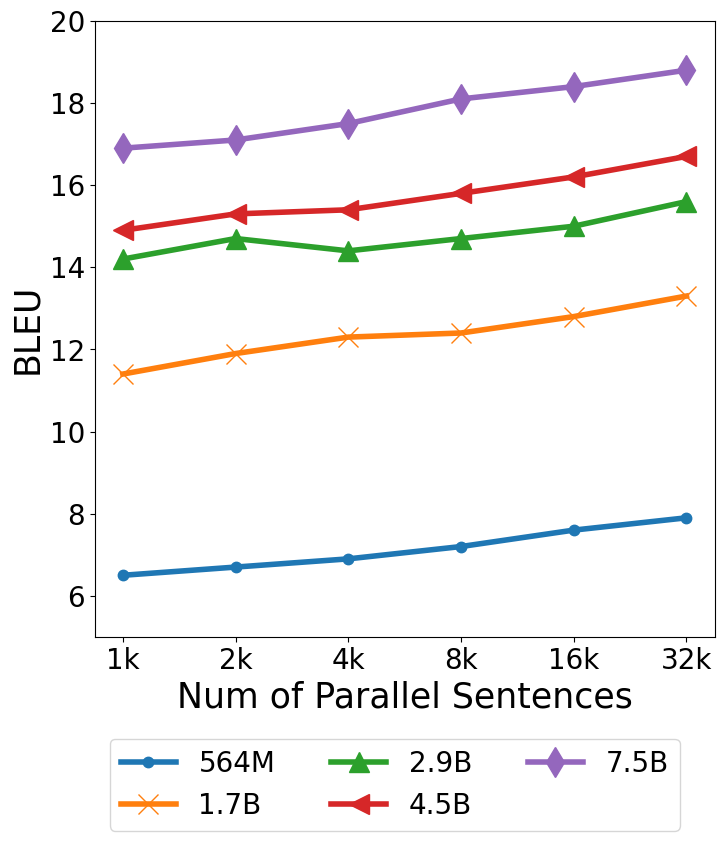
\includegraphics[width=0.85\linewidth]{figs/scaling.png}
\caption{The translation performance of finetuned XGLM as the number of model parameters and training examples scales.}
\label{fig:scaling}
\end{figure}



\paragraph{The Effectiveness of \method Scales with Model size and Training Examples.}
Figure \ref{fig:scaling} shows the translation performance when varying the number of training examples per language pair (1k, 2k, 4k, 8k, 16k, 32k) and the number of model parameters (564M, 1.7B, 2.9B, 4.5B, 7.5B). As we can see, it follows a standard log-linear scaling law in terms of both the number of training examples and model size, which is consistent with findings in the previous work \citep{kaplan2020scaling}.




